\section{G\'en\'eralit\'es sur l'interaction laser-atome en champ fort}

\begin{frame}
 \frametitle{Progression}
 \framesubtitle{}
 \begin{itemize}
   \item \textcolor{gray}{Introduction}
   \item \textbf{G\'en\'eralit\'es sur l'interaction laser-atome
en champ fort}
   \item Nouvelle approche de r\'esolution
dans l'espace des moments
   \item R\'esultats
   \item Conclusion
 \end{itemize}
\end{frame}

\begin{frame}
\frametitle{G\'en\'eralit\'es sur l'interaction laser-atome en champ fort}
\framesubtitle{Description du champ laser}

%\begin{textblock*}{100pt}(280pt,145pt)
%\includegraphics[scale=.3]{SphericalConventionalHarpyeagle-0.png}
%
%\end{textblock*}

%\begin{itemize}
% \item Equations de Maxwell 
% \item Formulation du champ \`a l'aide des potentiels
% \item Jauges 
% \item Polarisation
%\end{itemize}


\begin{textblock*}{160pt}(30pt,60pt)
\begin{itemize}
\footnotesize
\item Equations de Maxwell dans le vide
\begin{equation*}
 \begin{split}
 \boldsymbol{\nabla} \times \boldsymbol{\mathcal{E}}
  & = -\frac{\partial}{\partial t}\boldsymbol{\mathcal{B}}, \qquad
     \boldsymbol{\nabla} \cdot \boldsymbol{\mathcal{E}}  = 0, \\
\boldsymbol{\nabla} \times \boldsymbol{\mathcal{B}}
  & =  \frac{1}{c^2}\frac{\partial}{\partial t} \boldsymbol{\mathcal E},\qquad
     \boldsymbol{\nabla} \cdot \boldsymbol{\mathcal{B}}  = 0,
\end{split}
\end{equation*}
\end{itemize}

\end{textblock*}



\begin{textblock*}{100pt}(250pt,70pt)
\footnotesize
\begin{equation*}
 \begin{split}
& \boldsymbol{\mathcal{E}} (\boldsymbol{r},t)
    = - \frac{\partial}{\partial t}\boldsymbol{A}(\boldsymbol{r},t)
      - \boldsymbol{\nabla}\Phi, \\
&  \boldsymbol{\mathcal{B}}  (\boldsymbol{r},t)
    = \boldsymbol{\nabla} \times \boldsymbol{A}(\boldsymbol{r},t).
      \label{eqn:field_pot_link}
\end{split}
\end{equation*}

\end{textblock*}

\begin{textblock*}{180pt}(30pt,130pt)
\footnotesize
\begin{itemize}
\item Equation d'onde
%\begin{equation*}
% \boldsymbol{A}(\boldsymbol{r},t)
%   = \sum_{\lambda}\,
%     \boldsymbol{\varepsilon}_{\boldsymbol{k}}  \left( q_\lambda\,
%     {\rm e}^{i(\boldsymbol{k}_\lambda\cdot\boldsymbol{r}
%         - \omega_\lambda t)}  + c.c \right)
%%     + q_\lambda^{\ast}\,\boldsymbol{\varepsilon}_{\boldsymbol{k}}^\ast
%%      {\rm e}^{-i(\boldsymbol{k}_\lambda\cdot\boldsymbol{r}
%%         - \omega_\lambda t)}
%    \label{eqn:quant_vec_pot},
%\end{equation*}

\end{itemize}

\end{textblock*}



\begin{textblock*}{180pt}(150pt,120pt)
\footnotesize
\begin{align*}
% \boldsymbol{A}(\boldsymbol{r},t)
%   = \sum_{\lambda}\,
%     \boldsymbol{\varepsilon}_{\boldsymbol{k}}  \left( q_\lambda\,
%     {\rm e}^{i(\boldsymbol{k}_\lambda\cdot\boldsymbol{r}
%         - \omega_\lambda t)}  + c.c \right)
%%     + q_\lambda^{\ast}\,\boldsymbol{\varepsilon}_{\boldsymbol{k}}^\ast
%%      {\rm e}^{-i(\boldsymbol{k}_\lambda\cdot\boldsymbol{r}
%%         - \omega_\lambda t)}
%    \label{eqn:quant_vec_pot},
& \partial_\mu \left( \partial^\nu A_\nu \right)
    - \Box A_\mu = 0  \quad \Longrightarrow \quad
 A_\mu \rightarrow A^\prime_\mu = A_\mu + \partial_\mu \chi,\qquad 
A_\mu = \left(\Phi,-\boldsymbol{A}\right) \\
& \mbox{\textbf{N\'ecessit\'e de fixation de la jauge}}
\end{align*}

\end{textblock*}

\begin{textblock*}{180pt}(30pt,150pt)
\footnotesize
\begin{itemize}
\item En champ fort 
\begin{align*}
 & I \gg 10^{12}\,{\rm W/cm^2}, \qquad\qquad I_0 = 3.51\times 10^{16}\,\rm W/cm^2,\\
 & \boldsymbol{A}(\boldsymbol{r},t) = A_0(t)\boldsymbol{\varepsilon}
 \cos (\boldsymbol{k}\cdot\boldsymbol{r}-\omega t + \phi),
   \qquad A_0(t)=A_0f(t), \qquad\qquad A_0 = \frac{1}{\omega}\sqrt{\frac{I}{I_0}}.
\end{align*}

\item Approximation dipolaire
\begin{equation*}
  \boldsymbol{k}\cdot\boldsymbol{r} \ll \omega t \qquad \Longrightarrow \qquad 
\boldsymbol{A}(t) = A_0(t)\boldsymbol{\varepsilon}
 \cos (\omega t + \phi).
\end{equation*}

\end{itemize}

\end{textblock*}



\end{frame}

\begin{frame}
\frametitle{G\'en\'eralit\'es sur l'interaction laser-atome en champ fort}
\framesubtitle{Description semi-classique de l'interaction rayonnement-mati\`ere}


\begin{textblock*}{200pt}(30pt,60pt)
\footnotesize
\begin{itemize}
\item Equation de Schr\"odinger en jauge vitesse
\begin{align*}
 &    i\frac{\partial}{\partial t} |\Psi\rangle
     =  H|\Psi\rangle, \\
& H = H_0
 + \frac{1}{2}\left(\boldsymbol{A}\cdot\boldsymbol{p}
  + \boldsymbol{p}\cdot\boldsymbol{A}\right)
   + \frac{1}{2}\boldsymbol{A}^2 +\Phi, \qquad\qquad 
H_0 = \frac{\boldsymbol{p}^2}{2} + V, \\
&\nabla\cdot\boldsymbol{A}=0, \qquad\Phi=0 \qquad\Longrightarrow\qquad
 H^{\rm v} = H_0
 + \boldsymbol{A}\cdot\boldsymbol{p}
   + \frac{1}{2}\boldsymbol{A}^2, 
\end{align*}
\item Transformations de jauge
\begin{align*}
& H^\prime  = {\rm e}^{i\chi} H {\rm e}^{-i\chi}
 - \frac{d\chi}{dt}, \qquad |\Psi^\prime\rangle = e^{i\chi}|\Psi\rangle
\end{align*}
\item Jauge longueur
\begin{align*}
& \chi = -\boldsymbol{A}\cdot\boldsymbol{r} \qquad\Longrightarrow\qquad
  H^{\rm l} = H_0 + \boldsymbol{\mathcal{E}}\cdot\boldsymbol{r}
\end{align*}
%Jauge longueur \\
%R\'ef\'erentiel de Kramers-Henneberger
\end{itemize}

\end{textblock*}


%\begin{textblock*}{150pt}(200pt,160pt)
%\footnotesize
%\begin{align*}
%\end{align*}
%
%\end{textblock*}
%\begin{itemize}
%\item Approximation dipolaire
%\item Transformations de jauge
%\item Approximation du champ fort
%\end{itemize}

\end{frame}


\begin{frame}
\frametitle{G\'en\'eralit\'es sur l'interaction laser-atome en champ fort}
\framesubtitle{Processus d'ionisations multiphotoniques}

\begin{textblock*}{200pt}(30pt,70pt)
\footnotesize
 \begin{itemize}
\item Param\`etre de Keldysh et potentiel pond\'eromoteur
\begin{equation*}
 \gamma = \sqrt{\frac{I_p}{2U_p}}, \qquad\ U_p = \frac{\mathcal{E}^2}{4\omega^2},
\end{equation*}
 \end{itemize}

\end{textblock*}


\begin{textblock*}{100pt}(270pt,45pt)
\begin{figure}[!htbp]
\centering
\scalebox{.45}{
\begin{tikzpicture}
%  \tikz \draw[help lines] (0, 0) grid (5, 5);
%%flat lines
  \draw[line width=2pt] (3,0) -- (5,0);  \draw[line width=2pt] (3,4) -- (5,4);
  \draw[line width=2pt] (6,0) -- (8,0);  \draw[line width=2pt] (6,4) -- (8,4);
  \draw[line width=2pt] (9,0) -- (11,0); \draw[line width=2pt] (9,4) -- (11,4);

%%vert lines
  \draw[->, line width=1.5pt] (4,0) -- (4,5);

  \draw[->, line width=1.5pt] (7,0) -- (7,1);     
  \draw[->, line width=1.5pt] (10,0) -- (10,1);

  \draw[->, line width=1.5pt] (7,1) -- (7,2);     
  \draw[->, line width=1.5pt] (10,1) -- (10,2);

  \draw[->, line width=1.5pt] (7,2) -- (7,3);     
  \draw[->, line width=1.5pt] (10,2) -- (10,3);
  \draw[->, line width=1.5pt] (7,3) -- (7,4);     
  \draw[->, line width=1.5pt] (10,3) -- (10,4);

  \draw[->, line width=1.5pt] (7,4) -- (7,5);     
  \draw[->, line width=1.5pt] (10,4) -- (10,5);

  \draw[->, line width=1.5pt] (10,5) -- (10,6);

%% braces
  \draw[snake=brace] (3.0,0.1) -- (3.0,3.9);
  \draw[snake=brace, mirror snake] (4.2,0) -- (4.2,5);
  \draw[snake=brace, mirror snake] (7.2,0) -- (7.2,5);
  \draw[snake=brace, mirror snake] (10.2,0) -- (10.2,6);

%%labels 
  \draw[] (4,-1)  node {(a)};   \draw[] (4.7,2.5) node {$\omega^\prime$};
  \draw[] (7,-1)  node {(b)};   \draw[] (7.7,2.5) node {$n\omega$};
  \draw[] (10,-1) node {(c)};   \draw[] (11.1,2.5) node {$(n+s)\omega$};
  \draw[] (5.5,.5) node {fondamental};   
  \draw[] (8.5,4.5) node {continuum};
  \draw[] (2.5,1.95) node {$I_p$};
%  \draw (0,0) grid (4,3);
\end{tikzpicture}
}
\end{figure}

\end{textblock*}

\begin{textblock*}{100pt}(250pt,145pt)
\begin{figure}[!htbp]
\centering
\scalebox{.45}{
 \subfloat[]{
 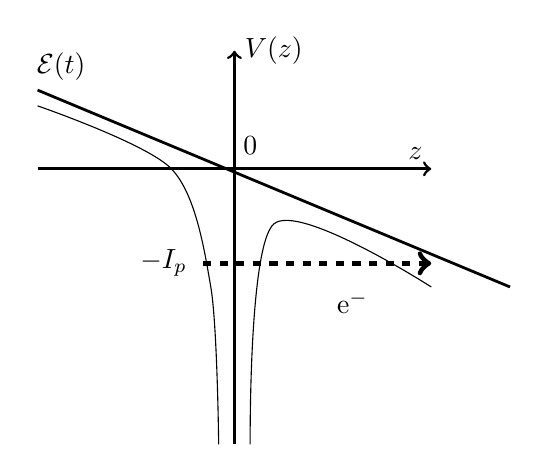
\begin{tikzpicture}
%% flat lines
  \draw[->,line width=1pt] (-6,0) -- (-1,0);

%% vert lines
  \draw[->,line width=1pt] (-3.5,-3.5) -- (-3.5,1.5);

  \draw[->,dashed,line width=2pt] (-3.9,-1.2) -- (-1,-1.2);
%%
  \draw[line width=1pt] (-6,1) -- (0,-1.5);

%% nodes
  \draw[] (-4.4,-1.2)  node {$-I_p$};  \draw[] (-2,-1.7) node {${\rm e}^-$};
  \draw[] (-3.,1.5)  node {$V(z)$};  \draw[] (-1.2,0.2) node {$z$};
  \draw[] (-3.3,.3)  node {$0$};
  %\draw[] (-3.5,-4.5)  node {a)};
  \draw[] (-5.7,1.3)  node {$\mathcal{E}(t)$};

%% parabolas
  %\draw[] (-6,.5) to[out=-10,in=100] (-3.8,-3.5);
  \draw[] plot [smooth] coordinates {(-6,0.8) (-4.3,-0)(-3.8,-1.5) (-3.7,-3.5)};
  \draw[] plot [smooth] coordinates {(-3.3,-3.5) (-3.0,-0.7) (-1,-1.5)};
\end{tikzpicture}
 \label{fig:tunnela}
}\;\;\;\;\;\;
 \subfloat[]{
  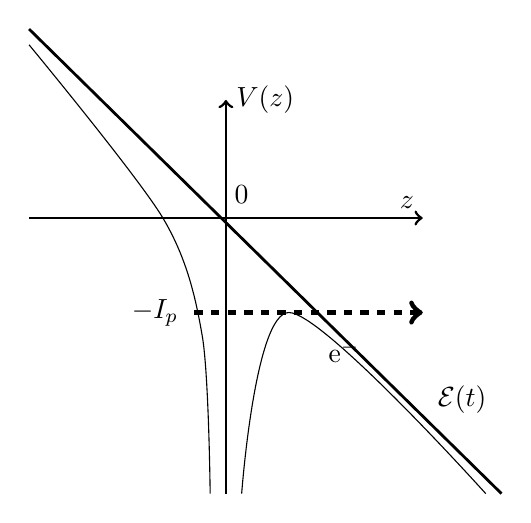
\begin{tikzpicture}
  \draw[->,line width=1pt] (1,0) -- (6,0);

  \draw[->,line width=1pt] (3.5,-3.5) -- (3.5,1.5);

  \draw[->,dashed,line width=2pt] (3.1,-1.2) -- (6,-1.2);

  \draw[line width=1pt] (1,2.4) -- (7,-3.5);

  %nodes
  \draw[] (2.6,-1.2)  node {$-I_p$};  \draw[] (5,-1.7) node {${\rm e}^-$};
  \draw[] (4.,1.5)  node {$V(z)$};  \draw[] (5.8,0.2) node {$z$};
  \draw[] (3.7,.3)  node {$0$};
  %\draw[] (3.5,-4.5)  node {b)};
  \draw[] (6.5,-2.3)  node {$\mathcal{E}(t)$};

  %parabolas
  \draw[] plot [smooth] coordinates {(1,2.2) (2.7,-0)(3.2,-1.5) (3.3,-3.5)};
  \draw[] plot [smooth] coordinates {(3.7,-3.5) (4.3,-1.2) (6.8,-3.5)};
 \end{tikzpicture}
 \label{fig:tunnelb}
}}
% \caption{Repr\'esentation sch\'ematique des deux possibilit\'es
%d'ionisation tunnel; a) ionisation tunnel normale;
% b) ionisation au-dessus de la barri\`ere}
%\label{fig:tunnel}
\end{figure}

\end{textblock*}

\begin{textblock*}{250pt}(30pt,130pt)
\footnotesize
 \begin{itemize}
 \item $\gamma \gg 1 \Longrightarrow \mbox{ R\'egime multiphotonique }$ 
 \item $\gamma \ll 1 \Longrightarrow \mbox{ R\'egime tunnel }$ 
 \item $\gamma \sim 1 \, \Longrightarrow \mbox{ R\'egime interm\'ediaire }$ 
 \end{itemize} \par\vspace{.5cm}


\begin{textblock*}{200pt}(30pt,180pt)
\footnotesize
\begin{itemize}
\item[$\bullet$] Electrons directs \hspace{.7cm} ($E < 2U_p$)
\item[$\bullet$] Electrons rediffus\'es \hspace{.4cm} ($2U_p<E<10U_p$)
%\item G\'en\'eration d'harmonique
\end{itemize}

\end{textblock*}

\end{textblock*}

\end{frame}


%\begin{frame}
%\frametitle{G\'en\'eralit\'es sur l'interaction laser-atome en champ fort}
%\framesubtitle{Approximation du champ fort}
%
%
%\begin{textblock*}{150pt}(350pt,115pt)
%\scalebox{.6}{
%\begin{tikzpicture}
% %\node at (0,0) {};
% \fill (7,0) circle (2pt);
% \fill (6.30,0) circle (1pt);
%%\fill (6.5,1) circle (1pt);
%%\draw (6.30,0) to [bend left=45] (6.5,1);
%%\draw (6.5,1) to [bend left=45] (8,1.5);
%%\fill (8,1.5) circle (1pt);
% \draw (7,0) circle (20pt);
% \draw (7,0) circle (40pt);
%\draw [->,thick,snake=snake] (5,3) -- (6.28,0.1);
%%\draw [->,snake=snake] (6.,3) -- (7.50,1.5);
%%\draw [->,snake=snake] (7.7,3) -- (8,2.5);
% \draw[solid,thick,->] plot [smooth] coordinates {(6.3,0)(7.5,2.2)(9.5,3.2)(10,3.4)};
% \node at (7.5,2.4){1};
% \node at (9.5,1.4){2};
% \draw[densely dashed,thick,->] plot [smooth] coordinates {(6.3,0)(7.5,1.5)(9.5,3)(7.3,.15)(10,1)};
%% \draw[densely dotted,thick,->] plot [smooth] coordinates {(6.3,0)(5.5,-1.5)(4.5,-2)(5.3,-.15)};
%% \draw[dotted,->] plot [] coordinates {(5.3,-.15)(6.3,0)};
%%\draw[] (6.3,0) to[out=100,in=100] (6.3,.1);
%%\draw[->] (6.30,0) to [bend left=45] (10,2.5);
%% \node at (7,.5) {\includegraphics[width=.7\linewidth]{../figures/chap3/sturm_mom_variation_nn_nbar.eps}};
%\end{tikzpicture}
%}
%\end{textblock*}
%
%
%\begin{textblock*}{180pt}(30pt,60pt)
%\footnotesize
%\begin{itemize}
%\item Etats de Volkov
%\begin{align*}
%& i\frac{\partial}{\partial t}
%  \boldsymbol{\chi}^{\rm V}_{\boldsymbol{k}}(\boldsymbol{r},t)
%  = \frac{1}{2}\left(\boldsymbol{p} + \boldsymbol{A}\right)^2
%   \boldsymbol{\chi}^{\rm V}_{\boldsymbol{k}}(\boldsymbol{r},t), \qquad\qquad \boldsymbol{\chi}^{\rm V}_{\boldsymbol{k}}(\boldsymbol{r},t)
%   = (2\pi)^{-3/2}{\rm e}^{i\boldsymbol{k}\cdot\boldsymbol{r}}
%  {\rm e}^{iS(\boldsymbol{k},\boldsymbol{r},t)},
%\end{align*}
%\end{itemize}
%\end{textblock*}
%
%\begin{textblock*}{180pt}(30pt,110pt)
%\footnotesize
%\begin{itemize}
%\item Mod\`ele \`a trois \'etapes
%\end{itemize}
%\end{textblock*}
%
%
%\begin{textblock*}{300pt}(40pt,125pt)
%\scriptsize
%\begin{enumerate}
%\item Absorption de photons et acc\`es \`a un \'etat du continuum
%\item Retour vers le noyau atomique et \'emission d'une harmonique
%\item Rediffusion \'elastique vers le continuum 
%\end{enumerate}
%\end{textblock*}
%
%
%\begin{textblock*}{350pt}(40pt,165pt)
%\scriptsize
%\begin{itemize}
%\item[$\bullet$] Explique classiquement les processus multiphotoniques 
%\item[$\bullet$] Donne des r\'esultats qualitativement corrects pour 
%le r\'egime basse fr\'equence 
%\item[$\bullet$] Permet des temps de convergences tr\`es rapides
%\item[$\bullet$] \color{red}{\textbf{R\'esultats quantitativement en d\'esaccord avec l'exp\'erience}}
%\item[$\bullet$] \color{red}{\textbf{Largement incorrect au del\`a de l'approximation dipolaire}}
%\item[$\Longrightarrow$] \color{blue}{\textbf{Trouver un moyen efficace de r\'esoudre num\'eriquement l'ESDT dans l'espace des moments}}
%\end{itemize}
%\end{textblock*}
%
%
%\end{frame}


